\documentclass[conference]{IEEEtran}
% \usepackage{silence}
% \WarningFilter[newline]{latex}{Underfull}

\usepackage{booktabs}
\usepackage{float}
\usepackage{multirow}

\usepackage{ifpdf}
% Enable correct encoding
\ifpdf{}
    \usepackage[utf8]{inputenc}
\fi{}
\usepackage[T1]{fontenc}

\usepackage[pdftex]{hyperref} % Enable hyperlinks
% \hypersetup{hidelinks}

% Citations Package
\usepackage[
    backend=biber,
    style=ieee
]{biblatex}
\addbibresource{citations.bib}

\title{Deep Learning’s Potential --- Differentiating Between Images of Concepts
and Tangible Objects}


\author{%
    \IEEEauthorblockN{Pratik Bhusal}
    \IEEEauthorblockA{%
        pratik.bhusal@utdallas.edu\\
        \today
    }\\

    \IEEEauthorblockN{Max Xie}
    \IEEEauthorblockA{%
        max.xie@utdallas.edu\\
        \today
    }
}

\usepackage{graphicx}


% 2. Report Presentation (40%): % {{{


%     1. Is the format correct? IEEE two-column style format, with the font name Times
%     New Roman and size 10.

%     2. Are there obvious grammatical errors or incomplete sentences?

%     3. Are there required sections missing? Each report should include title,
%     abstract, introduction, related work, one or more technical sections, one
%     section about empirical analysis, conclusion, and references.

%     4. Does the report contain plagiarism content?

%     5. Is the proposed AI algorithms and/or models described in sufficient detail?

%     6. What is an overall evaluation of the presentation?

%     7. Is there a clear description about the feature extraction process? Are
%     the features clearly described?

% % }}}

% 3. Technical content (50%): {{{

%     1. Does the implementation code include plagiarism content?

%     2. Is the code uploaded?

%     3. Is there any exploratory data analysis?

%     4. Are the research problem and the main tasks clearly described? The
%     students in one team should focus on separate tasks. If some students
%     focused on the same tasks, the differences of their contributions should be
%     described clearly.

%     5. What is the overall level of efforts for the main tasks. Each report
%     should clearly describe which parts of the code were written by the author.
%     The load of coding can be measured by the the time that is required to
%     implement and debug the code. This time will be estimated by the instructor
%     and TA based on an overall evaluation of the code.  If the load of coding is
%     too low (e.g., 2 hours), the level of efforts will be low (e.g, 0.2). If the
%     load of coding is high (e.g., 50 hours), the level of efforts will be high
%     (e.g., 0.9).

%     6. What is the level of originality and creativity about the proposed work?

%         Examples of high originality and creativity are: (1) The proposed work
%         replicates the results of an existing paper and conducts some new
%         empirical analysis not reported in the paper, such as empirical analysis
%         based on new evaluation metrics (e.g., area under curve, area under
%         precision-recall curve) and new datasets not considered in the paper.
%         (2) The proposed work conducts an empirical comparison between the
%         methods proposed in several different papers. (3) The proposed work
%         develops new algorithms or new neural network architectures and
%         demonstrates the effectiveness and/or efficiency of the proposed
%         techniques, in comparison with some baseline methods in real-world
%         datasets. Algorithms and neural network architectures modified from
%         existing ones are also considered as new. (4) The proposed work presents
%         novel applications of AI models that have not been studied in the
%         current literature. (5) The proposed work develops new algorithms and/or
%         models for Kaggle competitions and demonstrates the effectiveness and/or
%         efficiency of the proposed techniques on the kaggle datasets, in
%         comparison with some baseline methods.

%         Examples of low/medium originality and creativity: (1) The proposed work
%         only replicates the results of an existing paper but does not conduct
%         any new empirical analysis. (2) The proposed work implements classic AI
%         models (e.g., logistic regression, linear regression, bayesian neural
%         networks, support vector machines) for classic problems (e.g.,
%         classification, regression) on some benchmark datasets.

% 7. Is there a detailed discussion about how the hyper parameters were turned?
% Have the finalized hyperparameters of all the AI models been reported?

% 8. Are the empirical results discussed in sufficient detail?

% % }}}

\begin{document}
\maketitle

\begin{abstract} % {{{

% TODO: Write this section last. A reasonable way to write an abstract is to
% write a 1 sentence highlight of each of the sections in the paper, then go
% back and smooth it out so it flows cleanly and makes the key points you want.
% <2020-04-09, Pratik Bhusal>

Hello World
\end{abstract} % }}}



\section{Introduction} % {{{


% }}}



\section{Related Work} % {{{




\subsection{Training}\label{miniBatchSGD} % {{{

% TODO: Briefly mention mini batch SGD (Stochastic Gradient Descent), then
% politely point out some of it’s limitations. <2020-04-09, Pratik Bhusal>

Stochastic gradient descent (SGD) is one of the classical weight update rules
for neural networks. Using standard gradient descent as its foundation, SGD
takes random samples of batch size 1 and computing the gradient upon that sample
for each iteration. Depending on the original number of items in the batch, it
can significantly lower the overall MACs required in the model's training
step. However, this leads to the possibility of noisy weight updates that could
impede the network's optimization.

To counteract the SGD's greatest problem, mini-batch SGD takes slightly larger
batch sizes to reduce the noisy results and to maintain a lower MAC count in
comparison to a complete, standard gradient descent algorithm.

While mini-batch SGD is applicable to many applications and is able to avoid
saddlepoints, it still has its limitations. Because it is still based off of
SGD, mini-batch SGD still suffers from n-dimensional plateaus and cliffs.
Plateaus derive to a near 0 gradiant value making it difficult to train upon.
Cliffs have the opposite problem --- the gradients are too large to smoothly
optimize the model. The design section  will discuss how to amend such issues
and even converge faster than SGD\@.


% }}}


% }}}



\section{Design} % {{{

% TODO: Describe your new network design focusing on the encoder (body) building
% block structure and efficient for classification decoder (head). Provide some
% motivation and benefits, consider providing figures to illustrate key parts
% and a table to summarize the resulting family of designs.
% <2020-04-09, Pratik Bhusal>

\subsection{Depthwise Separable Convolutions}\label{subsec:depthwiseSeparableConvolutions} % {{{

To extarct strong features in an image classification task, 2-D convolution
layers are used in the encoder of the model. As the data goes through the
network, the weak features found in the original image become more pronounced
as the receptive field size and thus the number of feature maps increases.
Figure~\ref{fig:standard2DConvolution} depicts how a standard convolution takes
place in a 3$\times$3$\times$3 region gets convolved with a 3$\times$3$\times$3
to generate a 1$\times$1 receptive field of the output.

\begin{figure}[H]
    \centering
    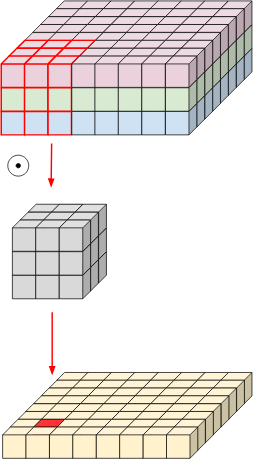
\includegraphics[height=50ex]{./figures/standardConvolution.png}
    \caption{Standard 2D Convolution~\cite{depthWiseConvolutionImages}}\label{fig:standard2DConvolution}
\end{figure}

However, because we are mixing across \textit{and} within channels, there is a
high computational complexity for each convolution. To remedy this issue, we
split the mixings into 2 insolated steps.  First, depth-wise convolution is applied.

\begin{figure}[H]
    \centering
    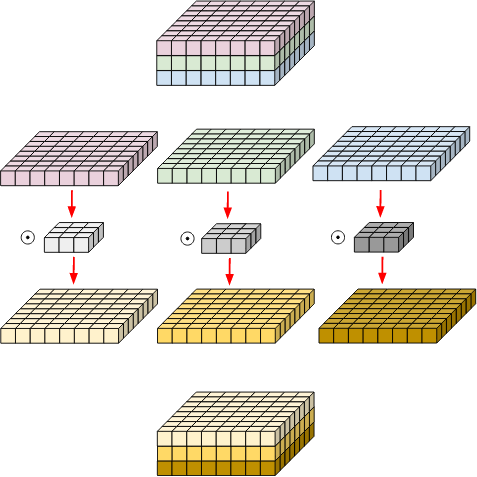
\includegraphics[height=50ex]{./figures/depthWiseConvolution.png}
    \caption{Depth-Wise Convolution~\cite{depthWiseConvolutionImages}}%
    \label{fig:depthWiseConvolution}
\end{figure}

Each channel is convolved separately in Figure~\ref{fig:depthWiseConvolution}.
Then, they are stacked thereafter to complete the intermediate step of depthwise
separable convolutions. This intermediate phase is where ``mixing within
channels'' occurs. Next, pointwise convolution is applied.


\begin{figure}[H]
    \centering
    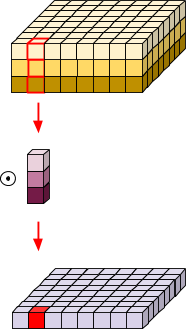
\includegraphics[height=50ex]{./figures/depthWiseSeparableConvolution.png}
    \caption{Depth-Wise Convolution~\cite{depthWiseConvolutionImages}}%
    \label{fig:depthWiseSeparableConvolution}
\end{figure}


Figure~\ref{fig:depthWiseSeparableConvolution} depicts the final phase of ``mixing
across channels''. A point wise convolution is applied to each
1$\times$1$\times$3 region to generate the same result as a standard 2D
convolution layer.

By using this design for convolutions, it greatly reduces the number of
trainable parameters~\cite{mobile_net_paper}.

\begin{equation}
    \frac{1}{N} + \frac{1}{D_k^2}
    \label{eq:depthwiseSeparableConvolutionEquation}
\end{equation}

Equation~\ref{eq:depthwiseSeparableConvolutionEquation} empherically defines the
computational cost reduction of depthwise separable convolutions. Here,
\textit{N} represents the number of output feature maps and $D_K^2$ represents
the demensions of the filter.

% }}}


\subsection{Inverted Residual Bottleneck Blocks} % {{{

This block structure uses the depthwise separable convolutions defined in the
previous scection~\ref{subsec:depthwiseSeparableConvolutions}. These blocks
provide a middle ground between the complexity of deeper networks while also
keeping some of the simplicity and computational ease of shallower network
designs. Most importantly, they help overcome the limitations of mini-batch SGD
implementations mention in
Section~\ref{miniBatchSGD}.Figure~\ref{fig:invertedResidualBottleneckBlock}
provides a visual example of the residual bootleneck block.


\begin{figure}[H]
    \centering
    \resizebox{\linewidth}{!}{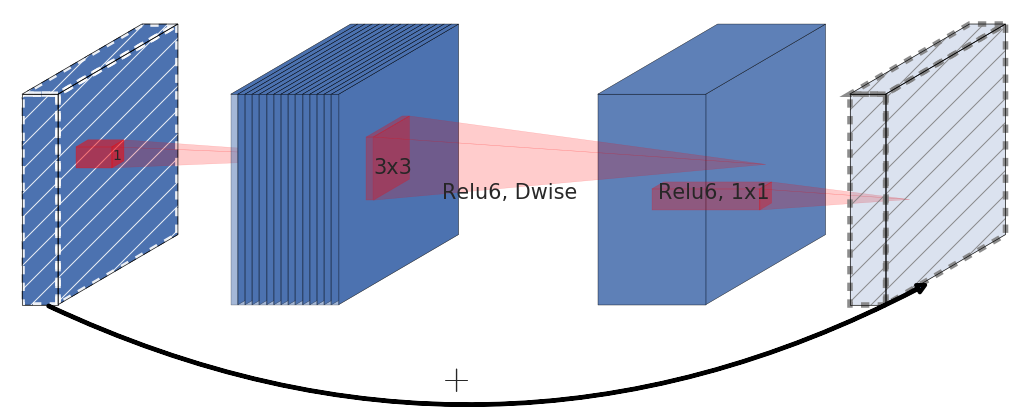
\includegraphics{./figures/inverted_residual.png}}
    \caption{Inverted Residual BottleNeck
    Block~\cite[p. 3]{mobile_net_v2_paper}}\label{fig:invertedResidualBottleneckBlock}
\end{figure}

The ``inversion'' comes from the fact that we create an expansion bottleneck. By
increasing the number of feature maps by an expansion factor $t$ before we
perform depth wise convolutions. Now, only a select few channels pass into a
depthwise separable convolution block.

Finally, a residual connection is added together to the output of the depthwise
separable convolution block to get the final output of the inverted residual
bottleneck block. By doing so it helps with the propagation of the output of the
depthwise separable convolution block and thus alleviates the issue of vanishing
and exploding gradients~\cite{inverted_residual_bottleneck_blocks}. With this
implementation, it keeps the number of channels low while also maintaining a
high accuracy~\cite{mobile_net_v2_paper}.

% }}}


\subsection{Architecture Overview} % {{{

The following subsections go into deatail of the Encoder-Decoder style
architecture of MobileNet. This is the reference point for the CIFAR-10
implementation itself will be based off of and is heavily inspired by a paper of
a similar design~\cite{mobile_net_v2_paper}.  This particular model has
1,184,746 trainable parameters. Some noteworthy points are that the
ReLU-6 activation function is used instead of standard ReLU to allow learning
sparse features.  ReLU-6 can be defined as $\min(6, ReLU(\textbf{x}))$.

% }}}


\subsection{Encoder --- Tail Architecture} % {{{

\begin{table}[H]
    \centering
    \resizebox{\linewidth}{!}{\begin{tabular}{@{}ccccccc@{}}
        \toprule
        & \multicolumn{2}{c}{Input Dimensions} \\
        \cmidrule{2-3}
        Layer  & Feature Map & Size & \multirow{-2}{10ex}{\centering Expansion
        Factor} & Repeats & Stride & \multirow{-2}{9ex}{\centering Output
        Channels}\\
        \midrule

        Image       & 3 & 28$\times$28 & --- & --- & --- & --- \\
        Convolution & 3 & 28$\times$28 & --- & 1   & 1   & 32  \\

        \bottomrule\smallskip
    \end{tabular}}\caption{MobileNet V2 tail for CIFAR 10
    dataset.}\label{table:MobileNetCifar10TailArchitecture}
\end{table}

The single 2D convolution layer exists to match the number of output feature
maps with the input to the first residual bottleneck block. It also provides the
beginning of the feature extraction propagation for the remainder of the body.

% }}}


\subsection{Encoder --- Body Architecture} % {{{

\begin{table}[H]
    \centering
    \resizebox{\linewidth}{!}{\begin{tabular}{@{}ccccccc@{}}
        \toprule
        & \multicolumn{2}{c}{Input Dimensions} \\
        \cmidrule{2-3}
        Layer  & Feature Map & Size & \multirow{-2}{10ex}{\centering Expansion
        Factor} & Repeats & Stride & \multirow{-2}{9ex}{\centering Output
        Channels}\\
        \midrule

        Residual Bottleneck & 32  & 28$\times$28 & 6 & 4 & 2 & 64  \\
        Residual Bottleneck & 64  & 14$\times$14 & 6 & 3 & 1 & 96  \\
        Residual Bottleneck & 96  & 14$\times$14 & 6 & 3 & 2 & 160 \\
        Residual Bottleneck & 160 & 7$\times$7   & 6 & 1 & 1 & 320 \\

        \bottomrule\smallskip
    \end{tabular}}\caption{MobileNet V2 body for CIFAR 10
    dataset.}\label{table:MobileNetCifar10BodyArchitecture}
\end{table}

The body contains the residual bottleneck blocks. We  repeat each block a cetain
amount of times and then downsample to the next layer in the network. Note that
each residual block has 3 layers to compute to. They are not shown in
Table~\ref{table:MobileNetCifar10BodyArchitecture} for brevity.

% }}}


\subsection{Decoder --- Head Architecture} % {{{

\begin{table}[H]
    \centering
    \resizebox{\linewidth}{!}{\begin{tabular}{@{}ccccccc@{}}
        \toprule
        & \multicolumn{2}{c}{Input Dimensions} \\
        \cmidrule{2-3}
        Layer  & Feature Map & Size & \multirow{-2}{10ex}{\centering Expansion
        Factor} & Repeats & Stride & \multirow{-2}{9ex}{\centering Output
        Channels}\\
        \midrule

        Global Average Pool & 320 & 7$\times$7 & --- & 1 & --- & --- \\
        Dense (softmax)     & 1   & 320        & --- & 1 & --- & 10  \\

        \bottomrule\smallskip
    \end{tabular}}\caption{MobileNet V2 head for CIFAR 10
    dataset.}\label{table:MobileNetCifar10HeadArchitecture}
\end{table}

Finally, the decoder takes in the encoded information and categorises the strong
features derived fromt he encoder and passed it to a global average pooling
layer followed by a fully connected layer to get the most likely classification
for the given input image. A softmax operation is applied to transform the
output into a probability mass function.

% }}}



% }}}



\section{Training} % {{{

% TODO: Describe your new training methods. Include a figure with training data
% loss and validation data accuracy curves. Mention different experiments you
% tried and their results. <2020-04-09, Pratik Bhusal>

\subsection{Batch Normalization}

Internal covarience shift is always a concern when trying to have networks
converge as quickly and as efficiently as possible. It occurs during training
when the input distribution changes throughout the model. For neural networks in
particular, each layer's input is affected by the parameters of \textit{all}
other input layers. When there are significant differences in the results on a
per-batch level, the model will have a difficult time optimizing and converging
to a minima of error.

To combat the issues, we add another layer to our model after each convolution
layer that normalizes each feature map by their respective mean and
variance~\cite{batch_norm_paper}. This technique that normalizes the batches is
known as ``batch normalization'' (batch norm). Depending on the size of the
batches, the model generalizes more cleanly overall. Because of these
advantages, we do not need to use Dropout layers.

\subsection{Learning Rate Scheduling}

\begin{figure}[H]
    \centering
    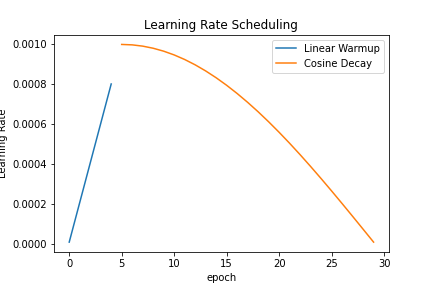
\includegraphics[width=0.8\linewidth]{figures/learning_rate_scheduling.png}
    \caption{Learning Rate Scheduling}\label{fig:learning_rate_scheduling}
\end{figure}

A slightly modified version of simulated anneling takes place with the learning
rate. As seen in Figure~\ref{fig:learning_rate_scheduling}, the initial learning
rate linearly increases until a certain threshhold is met. Once passed it, the
learning rate follows a cosine decay pattern to allow for the model to converge
to a local minima of error.

\subsection{RMSProp Optimizer}

Finally, instead of using mini-batch SGD, we utilize the RMSProp optimizer. In
essence it still calculates gradiends similar to mini-batch SGD, but it tracks an
average of the square of the calculated gradients. When taking the square roots
of these stored values, we mitigate the magnitue of the weight update and
prioritize the direction of convergence more than how much the model has moved.

% }}}



\section{Conclusion} % {{{

% TODO: Write 1 – 2 sentences on each of motivation, design, training and
% implementation. Do this after putting together the other sections but before
% the abstract. <2020-04-09, Pratik Bhusal>

MobileNet V2 is a new take on neural network design that is optimized for mobile
and embedded systems. Using new techniques such as inverted residuals, depth
wise convolution, learning rate scheulding, and batch normalization help in not
only keeping the amount of computations low but also maintaining a high
accuracy. The experiments shown have provided validation accuracy results that
far exceed its contemporary models.

% }}}



{\hbadness=10000\printbibliography}

\end{document}
